\section{Introduction}\label{sec:intro}

Affective computing is an emerging interdisciplinary research field ranging from cognitive and social sciences to human computer interaction (HCI) researches with techniques like computer vision, machine learning, nature language understanding etc.

With the long-term research on emotion theory from psychology and neuroscience\cite{james1884emotion, turkle2005second}, emotion has been confirmed to be a significant effect \cite{james2013emotion} on human communication, decision making, perception and so on.

On the perspective of human computer interaction, Picard \cite{Picard1999} pointed out that affective computing involved projects can be used for \emph{reducing user frustration} enabling comfortable communication of user emotion, developing infrastructure and applications to \emph{handle affective information}, as well as building tools that \emph{help develop social-emotional skills}.

Recently, the ubiquitous computing and wearable computing, which are closely related to affective computing, have achieved the pervasive attention of scientists. Ubiquitous computing and wearable computing are the necessary products of the combination of mobile computing technology and computer individualization.

In this paper, we presents an introduction to the mobile affective computing techniques, our next section discusses the exists data source from mobile devices, and Section \ref{sec:methods} illustrate the recent advances for each different type of data and present the state-of-the-art model and method. Next, Section \ref{sec:applications} based on the previous information, we fairly assume we has finished user emotion inferring stage, then gives two typical HCI applications in this field. At last, Section \ref{sec:challenges} and \ref{sec:conclusion} discusses the current challenges of mobile affective inferring and our conclusion of this introduction.
Figure~\ref{fig:hierarchically} shows the hierarchically-structured taxonomy of this paper.

\begin{figure*}[htb]
    \centering
    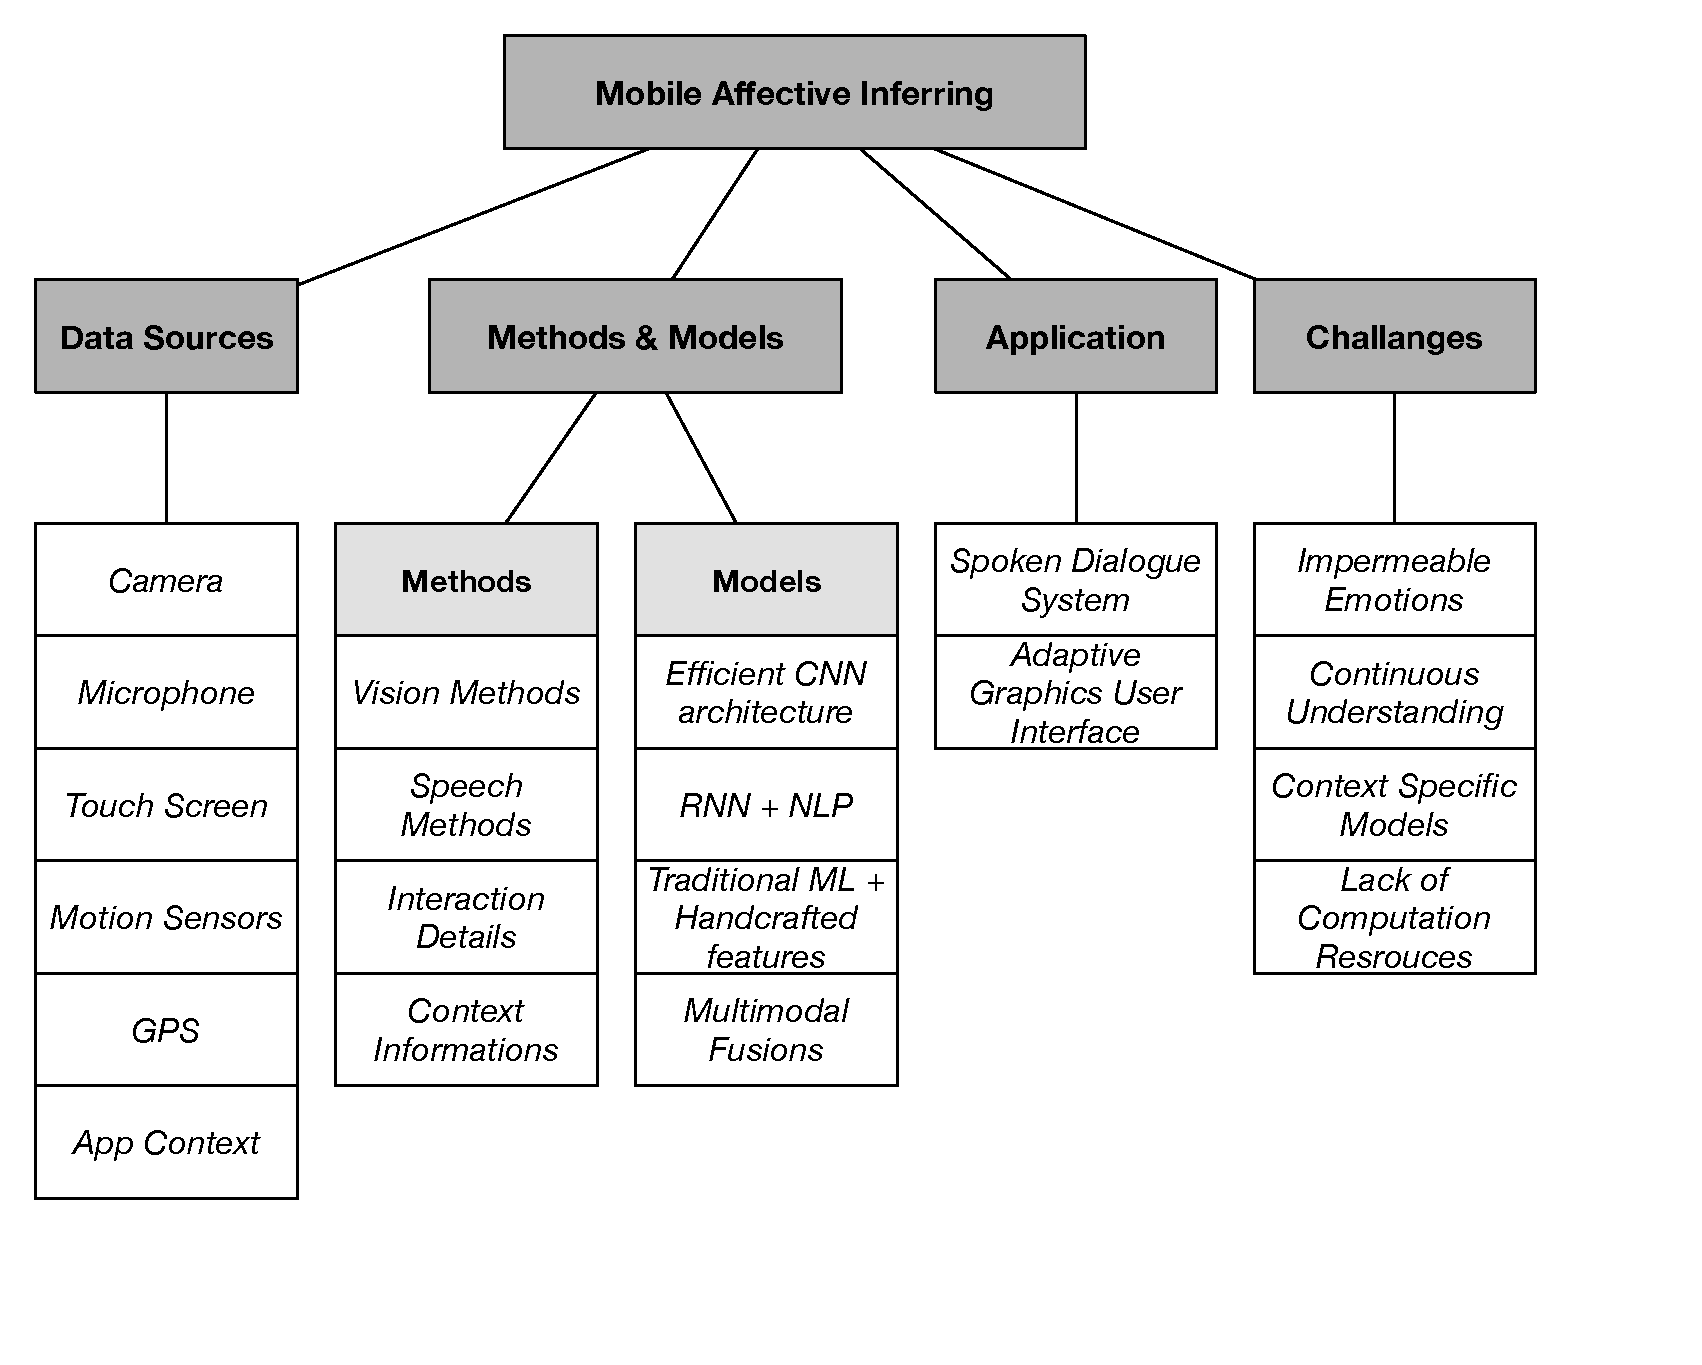
\includegraphics[width=\textwidth]{hierarchical}
    \caption{Hierarchically-structured taxonomy of this paper.}
    \label{fig:hierarchically}
\end{figure*}